%%%%%%%%%%%%%%%%%%%%%%%%%%%%%%%%%%%%%%%%%%%%%%%%%%%%%%%%%%%%%%%%%%%%%%%%%%%%%%%%
% DynBodyInit_spec.tex
% Toplevel specification of the Body Action Model
%
%%%%%%%%%%%%%%%%%%%%%%%%%%%%%%%%%%%%%%%%%%%%%%%%%%%%%%%%%%%%%%%%%%%%%%%%%%%%%%%%

\chapter{Product Specification}\label{ch:\modelpartid:spec}

\section{Conceptual Design}

The DynBody State Initialization Sub-Model comprises several classes that
provide various mechanisms for initializing the state
(position, velocity, attitude, and angular velocity) of
a DynBody object. All of the classes in this sub-model derive from
a single base class. The base class for initializing the state of a DynBody
object is the DynBodyInit class. The class inheritance for the sub-model
is depicted below.

\begin{figure}[H]
\begin{center}
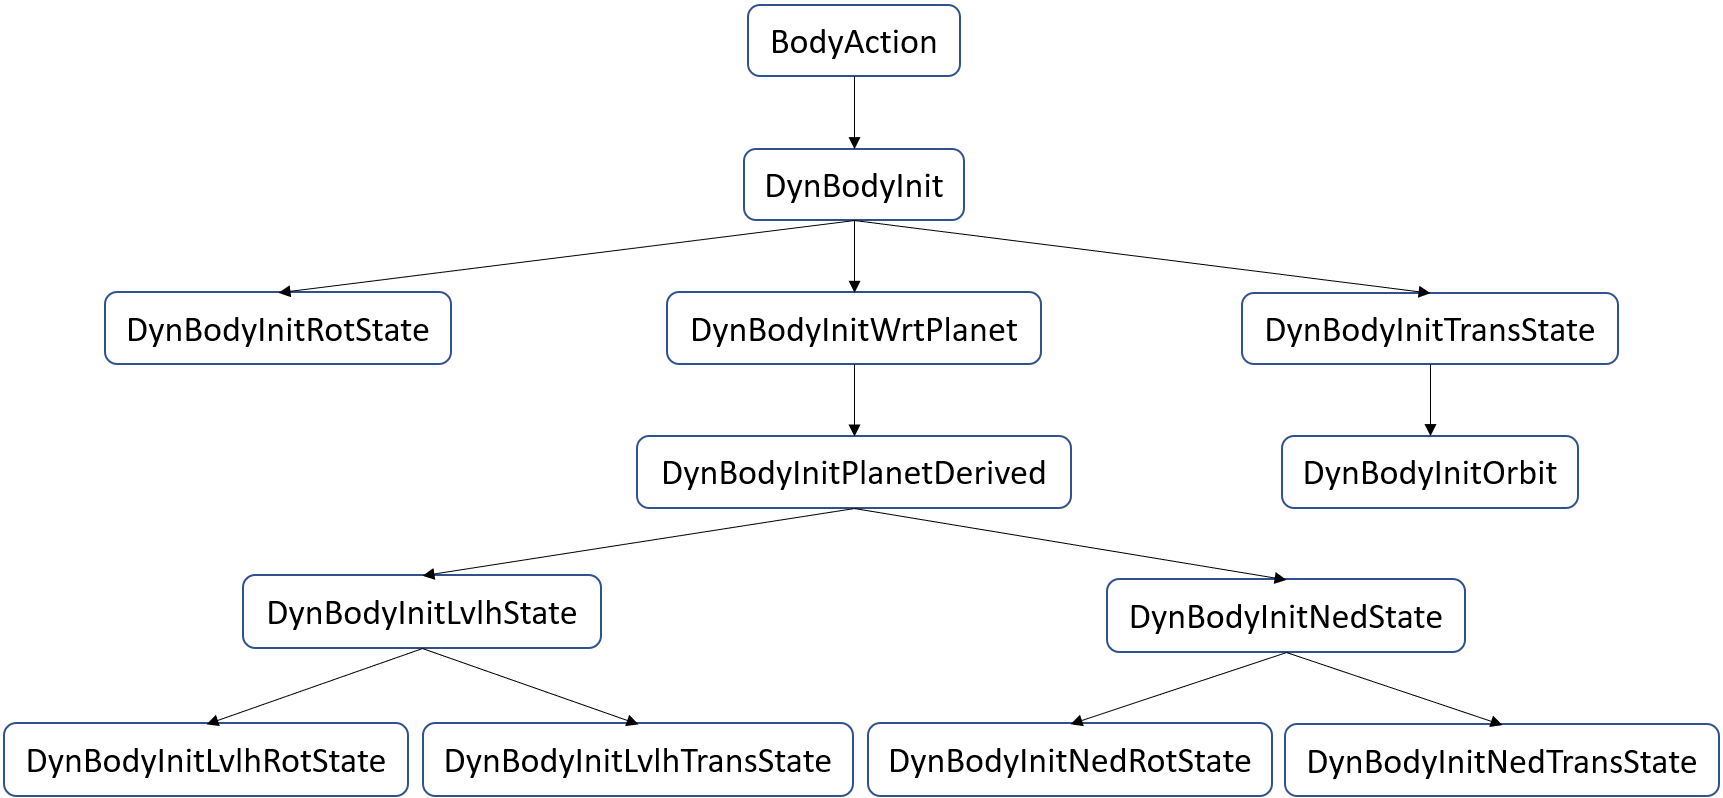
\includegraphics[width=\textwidth] {fig/fig1.png}
\end{center}
\end{figure}

\section{Mathematical Formulations}
Most of the classes defined in the DynBody State Initialization Sub-Model
rely on some other model to do all of the mathematical calculations.
The one exception is the DynBodyInitOrbit class. This class uses the
Orbital Elements Model to do most of the work in converting orbital elements
to position and velocity vectors. The Orbital Elements Model accepts but
one set of orbital elements. The DynBodyInitOrbit accepts seven sets.
Translating the data in those seven sets to the set accepted by the
Orbital Elements Model requires a bit of work\cite{Vallado}:

\begin{align}
  e \cos E &= \frac {a-r}{a} \\
  e \sin E &= \frac{r\dot r}{\sqrt{\mu a}} \\
  e^2 &= (e\cos E)^2 + (e\cos E)^2 \\
  k \cos \nu &= e \cos E - e^2 \\
  k \sin \nu &= \sqrt{1-e^2} e \sin E \\
  \tan \nu &= \frac{k \sin \nu}{k \cos \nu} \\
  \omega &= u - \nu \\
  a &= R_{\text{planet}} + (h_{\text{apo}} + h_{\text{peri}})/2 \\
  e &= \frac {(h_{\text{apo}} - h_{\text{peri}}}{2a} \\
  p &= a(1-e^2) \\
  M &= \frac{T_{\text{peri}}}{a} \sqrt{\frac {\mu}{a}}
\end{align}

\section{Detailed Design}

\subsection{Class DynBodyInit}
The base class for initializing the state of a DynBody object is DynBodyInit.

A DynBody has a minimum of three distinct reference frames:
\begin{itemize}
\item The structural frame, with origin at a fixed point on the vehicle
and reference frame axes defined with respect to the vehicle;
\item The core body frame, with origin at the core center of mass and
and reference frame axes a fixed rotation from the structural axes; and
\item The composite body frame, with origin at the composite center of mass and
and reference frame axes collinear with the core body frame axes.
\end{itemize}
Any given instance of a DynBodyInit object can specifically initialize elements
of one of those frames.

A DynBodyInit object contains the position, velocity, attitude, and
angular velocity of the subject reference frame with respect to some reference
reference frame. These state data form the primary user inputs to the
DynBodyInit object. (The DynBodyInitOrbit class ignores these inputs.)

The DynBodyInit class overrides the trio of virtual methods defined by the
the class BodyAction. It adds one new virtual method to this trio, the
{\tt initializes\_what()} method. This method specifies which of the elements
of the subject body frame are to be initialized. The default implementation
indicates that no elements of the subject body frame are to be initialized.
All derived classes must override this default, either directly or
by inheritance from some intermediate derived class.

\subsection{Derived Classes}
\begin{description}
\item[DynBodyInitRotState] Derives from DynBodyInit. \\
Instances of this class initialize a vehicle's attitude
and/or attitude rate.
\item[DynBodyInitTransState] Derives from DynBodyInit
Instances of this class initialize a vehicle's position
and/or velocity.
\item[DynBodyInitOrbit] Derives from DynBodyInitTransState. \\
Instances of this class initialize a vehicle's position
and velocity by means of some orbit specification.
\item[DynBodyInitPlanetDerived] Derives from DynBodyInitWrtPlanet,
which in turn derives from DynBodyInit. \\
These classes form the basis for subsequent derived classes that
initialize state with respect to a planetary frame.
\item[DynBodyInitLvlhState] Derives from DynBodyInitPlanetDerived. \\
Instances of this class initialize state with respect to the
rectilinear or curvilinear LVLH frame defined by some reference
vehicle's orbit about a specified planet.
Two derived classes from this class,
DynBodyInitLvlhRotState and DynBodyInitLvlhTransState,
limit the initialization to the rotational and translational
states of the subject DynBody.
\item[DynBodyInitNedState] Derives from DynBodyInitPlanetDerived. \\
Instances of this class initialize state with respect to the
North-East-Down frame defined by some reference vehicle or
reference point.
Two derived classes from this class,
DynBodyInitNedRotState and DynBodyInitNedTransState,
limit the initialization to the rotational and translational
states of the subject DynBody.
\end{description}
